\documentclass{article}
\usepackage[utf8]{inputenc}
\usepackage{geometry}
\usepackage{url}
\usepackage[utopia]{mathdesign}
\usepackage{tikz}
\usepackage{amsmath}
 \geometry{
 a4paper,
 total={170mm,257mm},
 left=20mm,
 top=20mm,
 }
 \usepackage{graphicx}
 \usepackage{titling}

 \title{Report for mechanics of soft bodies questions
}
\author{GU JUN}
\date{Nov 4th. 2024}
 
\usepackage{fancyhdr}
\setlength{\headheight}{12.49998pt}
\addtolength{\topmargin}{-0.49998pt}
\fancypagestyle{plain}{%  the preset of fancyhdr 
    \fancyhf{} % clear all header and footer fields
    \fancyfoot[R]{\thepage}
    \fancyfoot[L]{\thedate}
    \fancyhead[L]{Soft Robotics Home Assignment \#3}
    \fancyhead[R]{\theauthor}
}
\makeatletter
\renewcommand{\maketitle}{%
  \newpage
  \null
  \vskip 1em%
  \begin{center}%
  \let \footnote \thanks
    {\LARGE \@title \par}%
    \vskip 1em%
    %{\large \@date}%
  \end{center}%
  \par
  \vskip 1em}
\makeatother

\usepackage{lipsum}  
\usepackage{cmbright}

\begin{document}

\maketitle

\noindent\begin{tabular}{@{}ll}
    Student & \theauthor\\
\end{tabular}
% working principle, advantage, novelty, and what interests you.

\section*{Q1 - Problem statement}
A soft robot moves inside a smooth rigid tube. 
The robot body consists of a cylindrical soft tube 
(length $L$, outer radius $R$, inner radius $r$) 
and thin rigid plates attached to the both ends of the tube.
Young's modulus of the tube material is given by $E$.
Air pressure $P$ is applied inside the tube through its one end. 
Assume that the robot extends along its central axis alone and radial deformation is negligible. 
Let $L = 100 mm$, $R = 10 mm$, $r = 6 mm$, $E = 1.0 MPa$, and $P = 0.10 MPa$,
estimate the extensional deformation of the robot.
\subsection*{Solution}
Determine the cross-sectional area  A  of the tube:
Since the tube has an inner radius  r  and an outer radius  R , the cross-sectional area is the area of the annular section:

\begin{equation}
  A = \pi (R^2 - r^2)
\end{equation}
Plugging in the values:
\begin{equation}
  A = \pi \left(10^2 - 6^2\right) \, \text{mm}^2 = \pi (100 - 36) \, \text{mm}^2 = 64\pi \, \text{mm}^2
\end{equation}

Calculate the force  $F$  exerted by the internal pressure:
The force due to the internal pressure  $P$  is the product of  $P$  and the cross-sectional area  $A$:

\begin{equation}
  F = P \cdot A
\end{equation}
Using  $P = 0.10 \, \text{MPa}$ and  $A = 64\pi \, \text{mm}^2$ :

\begin{equation}
  F = 0.10 \times 64\pi \, \text{N} = 6.4\pi \, \text{N}
\end{equation}

Compute the extensional deformation  $\Delta L$  using Hooke’s Law:
In an elastic material, deformation can be calculated by:
\begin{equation}
  \Delta L = \frac{F \cdot L}{E \cdot A}
\end{equation}

Substituting the values:
\begin{equation}
  \Delta L = \frac{6.4\pi \times 100}{1.0 \times 64\pi} \, \text{mm}
\end{equation}

Simplifying, we find:

\begin{equation}
  \Delta L = \frac{640\pi}{64\pi} \, \text{mm} = 10 \, \text{mm}
\end{equation}


Final Answer

The extensional deformation  $\Delta L$  of the robot is estimated to be:
\begin{equation}
  \boxed{\Delta L = 10 \, \text{mm}}
\end{equation}
\newpage
\section*{Q2 - Problem statement}
Show inertia matrix $M$ and connection matrices $J_{\lambda}$, $J_{\mu}$ of the two-dimensional body below. 
Length of orthogonal sides of all isosceles right triangles is $1$.
Thickness of the two-dimensional body is $h = 2$ and its density is $\rho = 12$.
\begin{figure}[h]
  \centering
  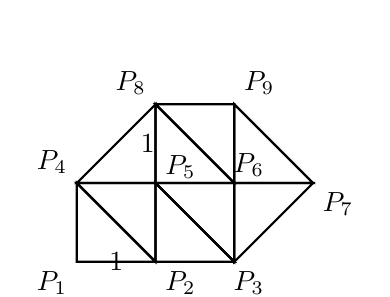
\begin{tikzpicture}
      % Coordinates for the points
      \coordinate (P1) at (0, 0);
      \coordinate (P2) at (1, 0);
      \coordinate (P3) at (2, 0);
      \coordinate (P4) at (0, 1);
      \coordinate (P5) at (1, 1);
      \coordinate (P6) at (2, 1);
      \coordinate (P7) at (3, 1);
      \coordinate (P8) at (1, 2);
      \coordinate (P9) at (2, 2);

      % Draw triangles
      \draw[thick] (P1) -- (P2) -- (P4) -- cycle;
      \draw[thick] (P2) -- (P4) -- (P5) -- cycle;
      \draw[thick] (P2) -- (P3) -- (P5) -- cycle;
      \draw[thick] (P3) -- (P5) -- (P6) -- cycle;
      \draw[thick] (P3) -- (P6) -- (P7) -- cycle;
      \draw[thick] (P6) -- (P7) -- (P9) -- cycle;
      \draw[thick] (P6) -- (P9) -- (P8) -- cycle;
      \draw[thick] (P5) -- (P6) -- (P8) -- cycle;
      \draw[thick] (P4) -- (P5) -- (P8) -- cycle;

      % Label the points
      \node[below left] at (P1) {$P_1$};
      \node[below right] at (P2) {$P_2$};
      \node[below left] at (2.5, 0) {$P_3$};
      \node[above left] at (P4) {$P_4$};
      \node[right] at (1, 1.2) {$P_5$};
      \node[below left] at (2.5, 1.5) {$P_6$};
      \node[below right] at (P7) {$P_7$};
      \node[above left] at (P8) {$P_8$};
      \node[above right] at (P9) {$P_9$};


      % Adding lengths on edges
      \node at (0.5, 0) {$1$};
      \node at (0.9, 1.5) {$1$};
  \end{tikzpicture}
\end{figure}

\subsection*{Solution}
We can first get $M_{i,j,k}$ for each triangle.\\
\begin{equation}
  M_{1,2,4}=M_{2,3,5}=M_{5,4,2}=M_{6,5,3}=M_{6,3,7}=M_{5,8,4}=M_{5,6,8}=M_{6,7,9}=M_{9,8,6}= \\
  \frac{\rho h \Delta}{12}\left[\begin{array}{ccc}
  2 l_{2 \times 2} & l_{2 \times 2} & l_{2 \times 2} \\
  l_{2 \times 2} & 2 l_{2 \times 2} & l_{2 \times 2} \\
  l_{2 \times 2} & l_{2 \times 2} & 2 l_{2 \times 2}
  \end{array}\right]
\end{equation}
\begin{equation*}
  \frac{\rho h \triangle}{12} = \frac{12 \times 2}{12} = 2
\end{equation*}
and\\
\begin{equation}
  \begin{aligned}
  M & =M_{1,2,4} \oplus M_{2,3,5} \oplus M_{5,4,2} \oplus M_{6,5,3} \oplus M_{6,3,7} \oplus M_{5,8,4} \oplus M_{5,6,8} \oplus M_{6,7,9} \oplus M_{9,8,6} \\
  & = 2 \left[\begin{array}{ccccccccc}
  2 l_{2 \times 2} & I_{2 \times 2} & & I_{2 \times 2} & & &\\
  l_{2 \times 2} & 6 l_{2 \times 2} & l_{2 \times 2} & 2 l_{2 \times 2} & 2 I_{2 \times 2} & & & \\
  & I_{2 \times 2} & 6 l_{2 \times 2} & & 2 l_{2 \times 2} & 2 I_{2 \times 2} & I_{2 \times 2} & & \\
  I_{2 \times 2} & 2 l_{2 \times 2} & & 6 I_{2 \times 2} & 2 I_{2 \times 2} & & & I_{2 \times 2}\\
  & 2 l_{2 \times 2} & 2 l_{2 \times 2} & I_{2 \times 2} & 10 l_{2 \times 2} & 2 I_{2 \times 2} & 2 I_{2 \times 2} & \\
  & & I_{2 \times 2} & & I_{2 \times 2} & 10 l_{2 \times 2} & 2 I_{2 \times 2} & 2 I_{2 \times 2} & 2 I_{2 \times 2} \\
  & & & & & 2 I_{2 \times 2} & 4 I_{2 \times 2} & & I_{2 \times 2} \\
  & & & I_{2 \times 2} & 2 I_{2 \times 2} & 2 I_{2 \times 2} & & 6 I_{2 \times 2} & I_{2 \times 2} \\
  & & & & & 2 I_{2 \times 2} & I_{2 \times 2} & I_{2 \times 2} & 4 I_{2 \times 2}
  \end{array}\right] .
  \end{aligned}
  \end{equation}
For $J_{\lambda}$, we need to calculate $J^{1,2,4}_{\lambda}$, $J^{2,3,5}_{\lambda}$, $J^{5,4,2}_{\lambda}$, $J^{6,5,3}_{\lambda}$, $J^{6,3,7}_{\lambda}$, $J^{5,8,4}_{\lambda}$, $J^{5,6,8}_{\lambda}$, $J^{6,7,9}_{\lambda}$, and $J^{9,8,6}_{\lambda}$.\\
For $J^{1,2,4}_{\lambda}$, we have:
\begin{equation}
  \boldsymbol{a}=\frac{1}{2 \triangle}\left[\begin{array}{l}
  y_j-y_k \\
  y_k-y_i \\
  y_i-y_j
  \end{array}\right]
  =\left[\begin{array}{l}
    -1 \\
    1 \\
    0
    \end{array}\right]
    \boldsymbol{b}= - \frac{1}{2 \triangle}\left[\begin{array}{l}
      x_j-x_k \\
      x_k-x_i \\
      x_i-x_j
      \end{array}\right]
      =\left[\begin{array}{l}
        -1 \\
        0 \\
        1
        \end{array}\right]
\end{equation}
then we can get:
\begin{equation}
  \begin{aligned}
  H_\lambda & =\left[\begin{array}{ll}
  \boldsymbol{a} \boldsymbol{a}^{\mathrm{T}} & \boldsymbol{a} \boldsymbol{b}^{\mathrm{T}} \\
  \boldsymbol{b} \boldsymbol{a}^{\mathrm{T}} & \boldsymbol{b}^{\mathrm{T}}
  \end{array}\right] h \triangle \\
  % H_\mu & =\left[\begin{array}{cc}
  % 2 \boldsymbol{a} \boldsymbol{a}^{\mathrm{T}}+\boldsymbol{b}^{\mathrm{T}} & \boldsymbol{b} \boldsymbol{a}^{\mathrm{T}} \\
  % \boldsymbol{a} \boldsymbol{b}^{\mathrm{T}} & 2 \boldsymbol{b} \boldsymbol{b}^{\mathrm{T}}+\boldsymbol{a}^{\mathrm{T}}
  % \end{array}\right] h \triangle
  H_\lambda & =\left[\begin{array}{ccc|ccc}
    1 & -1 & 0 & 1 & 0 & -1 \\
    -1 & 1 & 0 & -1 & 0 & 1 \\
    0 & 0 & 0 & 0 & 0 & 0 \\
    \hline 1 & -1 & 0 & 1 & 0 & -1 \\
    0 & 0 & 0 & 0 & 0 & 0 \\
    -1 & 1 & 0 & -1 & 0 & 1
    \end{array}\right]
  \end{aligned}
  \end{equation}
Because 1,4, 2, 5, 3, 6 rows and columns of $H_{\lambda}$ are 1, 2, 3, 4, 5, 6 rows and columns of $J^{1,2,4}_{\lambda}$.\\
\begin{equation}
  J_\lambda^{1,2,4}=\left[\begin{array}{rr|rr|rr}
  1 & 1 & -1 & 0 & 0 & -1 \\
  1 & 1 & -1 & 0 & 0 & -1 \\
  \hline-1 & -1 & 1 & 0 & 0 & 1 \\
  0 & 0 & 0 & 0 & 0 & 0 \\
  \hline 0 & 0 & 0 & 0 & 0 & 0 \\
  -1 & -1 & 1 & 0 & 0 & 1
  \end{array}\right]
  \end{equation}
We can do the same thing for $J^{2,3,5}_{\lambda}$, $J^{5,4,2}_{\lambda}$, $J^{6,5,3}_{\lambda}$, $J^{6,3,7}_{\lambda}$, $J^{5,8,4}_{\lambda}$, $J^{5,6,8}_{\lambda}$, $J^{6,7,9}_{\lambda}$, and $J^{9,8,6}_{\lambda}$.\\
And finally, we can get $J_{\lambda}$ by:
\begin{equation}
  \begin{aligned}
    J_{\lambda} & = J^{1,2,4}_{\lambda} \oplus J^{2,3,5}_{\lambda} \oplus J^{5,4,2}_{\lambda} \oplus J^{6,5,3}_{\lambda} \oplus J^{6,3,7}_{\lambda} \oplus J^{5,8,4}_{\lambda} \oplus J^{5,6,8}_{\lambda} \oplus J^{6,7,9}_{\lambda} \oplus J^{9,8,6}_{\lambda} \\
    & = \left[\begin{array}{cccccccccccccccccc}
            1 & 1 & -1 & 0 & 0 & 0 & 0 & -1 & 0 & 0 & 0 & 0 & 0 & 0 & 0 & 0 & 0 & 0 \\
            1 & 1 & -1 & 0 & 0 & 0 & 0 & -1 & 0 & 0 & 0 & 0 & 0 & 0 & 0 & 0 & 0 & 0 \\
            -1 & -1 & 2 & 1 & -1 & 0 & 0 & 1 & 0 & -1 & 0 & 0 & 0 & 0 & 0 & 0 & 0 & 0 \\
            0 & 0 & 1 & 2 & -1 & 0 & 1 & 0 & -1 & -2 & 0 & 0 & 0 & 0 & 0 & 0 & 0 & 0 \\
            0 & 0 & -1 & -1 & 1 & 0 & 0 & 0 & 0 & 1 & 0 & 0 & 0 & 0 & 0 & 0 & 0 & 0 \\
            0 & 0 & 0 & 0 & 0 & 2 & 0 & 0 & 1 & 0 & 0 & -2 & -1 & 0 & 0 & 0 & 0 & 0 \\
            0 & 0 & 0 & 1 & 0 & 0 & 2 & 0 & -2 & 0 & 0 & 0 & 0 & 0 & 0 & -1 & 0 & 0 \\
            -1 & -1 & 1 & 0 & 0 & 0 & 0 & 1 & 0 & 0 & 0 & 0 & 0 & 0 & 0 & 0 & 0 & 0 \\
            0 & 0 & 0 & -1 & 0 & 1 & -2 & 0 & 4 & 1 & -2 & -1 & 0 & 0 & 0 & 0 & 0 & 0 \\
            0 & 0 & -1 & -2 & 1 & 0 & 0 & 0 & 1 & 4 & -1 & 0 & 0 & 0 & 0 & -2 & 0 & 0 \\
            0 & 0 & 0 & 0 & 0 & 0 & 0 & 0 & -2 & -1 & 4 & 1 & -2 & 0 & 0 & 1 & 0 & -1 \\
            0 & 0 & 0 & 0 & 0 & -2 & 0 & 0 & -1 & 0 & 1 & 4 & 0 & 0 & 1 & 0 & -1 & -2 \\
            0 & 0 & 0 & 0 & 0 & -1 & 0 & 0 & 0 & 0 & -2 & 0 & 2 & 0 & 0 & 0 & 0 & 1 \\
            0 & 0 & 0 & 0 & 0 & 0 & 0 & 0 & 0 & 0 & 0 & 0 & 0 & 0 & 0 & 0 & 0 & 0 \\
            0 & 0 & 0 & 0 & 0 & 0 & 0 & 0 & 0 & 0 & 0 & 1 & 0 & 0 & 1 & 0 & -1 & -1 \\
            0 & 0 & 0 & 0 & 0 & 0 & -1 & 0 & 0 & -2 & 1 & 0 & 0 & 0 & 0 & 2 & 0 & 0 \\
            0 & 0 & 0 & 0 & 0 & 0 & 0 & 0 & 0 & 0 & -1 & 0 & 0 & -1 & 0 & 1 & 1 \\
            0 & 0 & 0 & 0 & 0 & 0 & 0 & 0 & 0 & 0 & -1 & -2 & 1 & 0 & -1 & 0 & 1 & 2
      \end{array}\right]\\
  \end{aligned}
\end{equation}
Similarly, we can get $J_{\mu}$ by:
\begin{equation}
  \begin{aligned}
    J_{\mu} & = J^{1,2,4}_{\mu} \oplus J^{2,3,5}_{\mu} \oplus J^{5,4,2}_{\mu} \oplus J^{6,5,3}_{\mu} \oplus J^{6,3,7}_{\mu} \oplus J^{5,8,4}_{\mu} \oplus J^{5,6,8}_{\mu} \oplus J^{6,7,9}_{\mu} \oplus J^{9,8,6}_{\mu} \\
    & = \left[\begin{array}{cccccccccccccccccc}
          3 & 1 & -2 & -1 & 0 & 0 & -1 & 0 & 0 & 0 & 0 & 0 & 0 & 0 & 0 & 0 & 0 & 0 \\
          1 & 3 & 0 & -1 & 0 & 0 & -1 & -2 & 0 & 0 & 0 & 0 & 0 & 0 & 0 & 0 & 0 & 0 \\
          -2 & 0 & 6 & 1 & -2 & -1 & 0 & 1 & -2 & -1 & 0 & 0 & 0 & 0 & 0 & 0 & 0 & 0 \\
          -1 & -1 & 1 & 6 & 0 & -1 & 1 & 0 & -1 & -4 & 0 & 0 & 0 & 0 & 0 & 0 & 0 & 0 \\
          0 & 0 & -2 & 0 & 4 & 0 & 0 & 0 & 0 & 1 & -2 & 0 & 0 & -1 & 0 & 0 & 0 & 0 \\
          0 & 0 & -1 & -1 & 0 & 5 & 0 & 0 & 1 & 0 & 0 & -4 & 0 & 0 & 0 & 0 & 0 & 0 \\
          -1 & -1 & 0 & 1 & 0 & 0 & 5 & 0 & -4 & 0 & 0 & 0 & 0 & 0 & 0 & 0 & 0 & 0 \\
          0 & -2 & 1 & 0 & 0 & 0 & 0 & 4 & 0 & -2 & 0 & 0 & 0 & 0 & -1 & 0 & 0 & 0 \\
          0 & 0 & -2 & -1 & 0 & 1 & -4 & 0 & 12 & 1 & -4 & -1 & 0 & 0 & -2 & 0 & 0 & 0 \\
          0 & 0 & -1 & -4 & 1 & 0 & 0 & -2 & 1 & 12 & -1 & -2 & 0 & 0 & 0 & -4 & 0 & 0 \\
          0 & 0 & 0 & 0 & -2 & 0 & 0 & 0 & -4 & -1 & 12 & 1 & -4 & 0 & 0 & 1 & -2 & -1 \\
          0 & 0 & 0 & 0 & 0 & -4 & 0 & 0 & -1 & -2 & 1 & 12 & 0 & -2 & 1 & 0 & -1 & -4 \\
          0 & 0 & 0 & 0 & 0 & 0 & 0 & 0 & 0 & 0 & -4 & 0 & 4 & 0 & 0 & 0 & 0 & 0 \\
          0 & 0 & 0 & 0 & -1 & 0 & 0 & 0 & 0 & 0 & 0 & -2 & 0 & 2 & 0 & 0 & 1 & 0 \\
          0 & 0 & 0 & 0 & 0 & 0 & 0 & -1 & -2 & 0 & 0 & 1 & 0 & 0 & 4 & 0 & -2 & 0 \\
          0 & 0 & 0 & 0 & 0 & 0 & 0 & 0 & 0 & -4 & 1 & 0 & 0 & 0 & 0 & 5 & -1 & -1\\
          0 & 0 & 0 & 0 & 0 & 0 & 0 & 0 & 0 & 0 & -2 & -1 & 0 & 1 & -2 & -1 & 4 & 1 \\
          0 & 0 & 0 & 0 & 0 & 0 & 0 & 0 & 0 & 0 & -1 & -4 & 0 & 0 & 0 & -1 & 1 & 5
        \end{array}\right]\\
  \end{aligned}
\end{equation}

\end{document}